\chapter{Viabilidad}
Este capítulo tiene como objetivo realizar, en base a los objetivos marcados en el capítulo anterior, elaborar un análisis de viabilidad del proyecto, analizando las diferentes tareas que contiene, calculando los correspondientes gastos y sus inherentes riesgos, que pueden afectar, atrasando o incluso impidiendo, la realización del proyecto.

\section{Requisitos funcionales del trabajo}
Los requisitos funcionales de la aplicación (RF a partir de ahora) se elaboran en base a los objetivos descritos y son los siguientes:

\begin{itemize}
	\item Elaborar un estado del arte que analice el campo de la seguridad informática, sus aplicaciones y analice el área del pentesting
	\item Elaborar una aplicación que permita obtener información sobre redes y nodos de la red
	\item Integrar correctamente herramientas de terceros para lograr que la aplicación resulte lo mas escalable posible.
	\item Aplicar principios sobre experiencia de usuario (UX) y sobre el diseño de interfaces gráficas (GUI) para que la aplicación sea lo mas sencilla y cómoda de usar
\end{itemize}

%------------------------------------------------------------------------------

\section{Planificación del tiempo}

\subsection[EDT]{Estructura de Descomposición del Trabajo}
El EDT, o Estructura del Desglose del Trabajo, es un sistema jerárquico que permite organizar las difernetes tareas de un proyecto. Es una técnica ámpliamnente usada para gestionar todo tipo de proyectos, especialmente proyectos de software.

A la hora de planificar el tiempo, se ha tenido en cuenta un enfoque en dos fases, a las cuales denominaremos Fase 1 y Fase 2. Esto es debido al carácter del proyecto. Por una parte, para elaborar la aplicación anteriormente mencionada, resulta fundamental realizar un estudio sobre el campo del la seguridad informática, mas concretamente sobre el área del pentesting, para poder llegar a encontrar las mejores herramientas y técnicas que permitan desarrollarla. Este estudio, bien desglosado y fundamentado, llevara a la obtención de un elaborado estado del arte, que sera el principal objetivo de la Fase 1. Además, dicha fase contiene un periodo de aprendizaje y familiarización con diversos conceptos y tecnologías, que también quedaran reflejados.

En la Fase 2, en función de lo aprendido en la Fase 1, se elaborará la aplicación en base a los criterios de implementar diversas utilidades junto a un experiencia de usuario (UX) óptima, que vendrá acompañada de un buen diseño de una interfaz gráfica (GUI).

El EDT completo quedaría tal y como se muestra en la figura \ref{fig:edt}.

\begin{landscape}
	
	\begin{figure}[H]
		\centering
		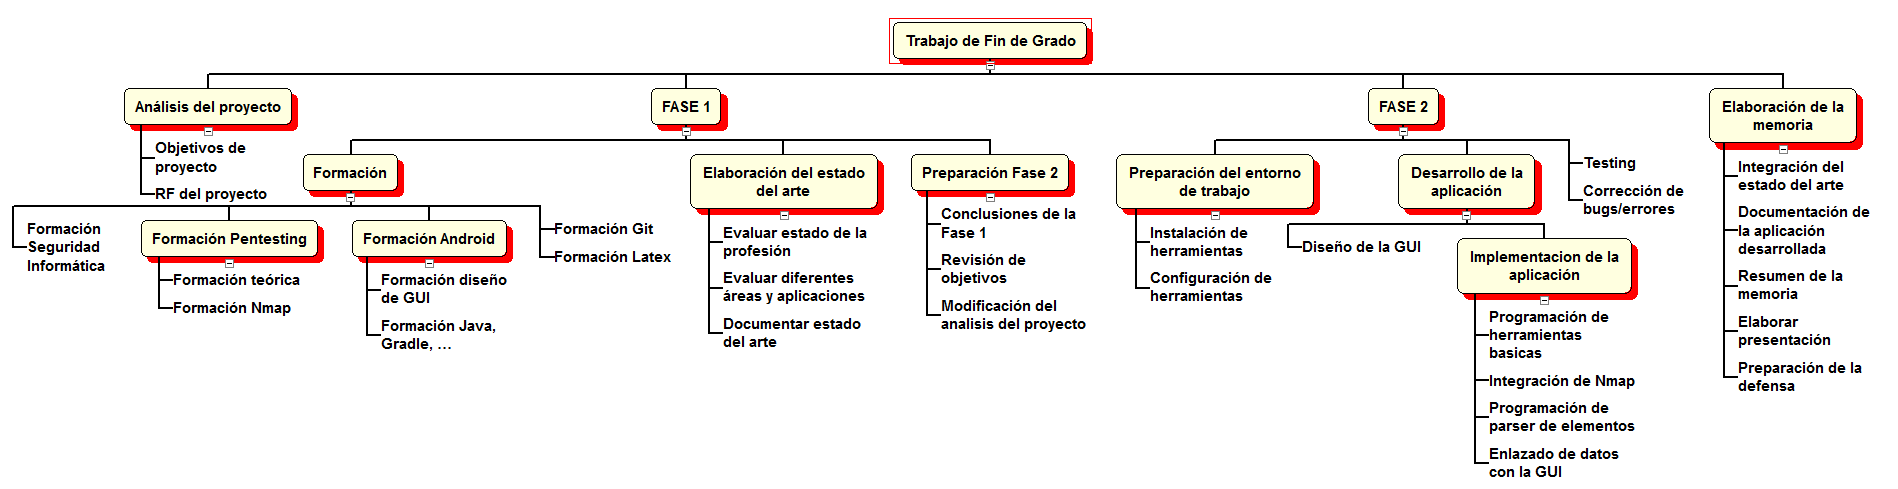
\includegraphics[height=150px]{TFG_EDT}
		\caption{EDT completo}
		\label{fig:edt}
	\end{figure}
	
	\clearpage
	
	\subsubsection{Fase 1}
	El EDT para la Fase 1 quedaría como se muestra en la figura \ref{fig:edt1}.
	
	\begin{figure}[H]
		\centering
		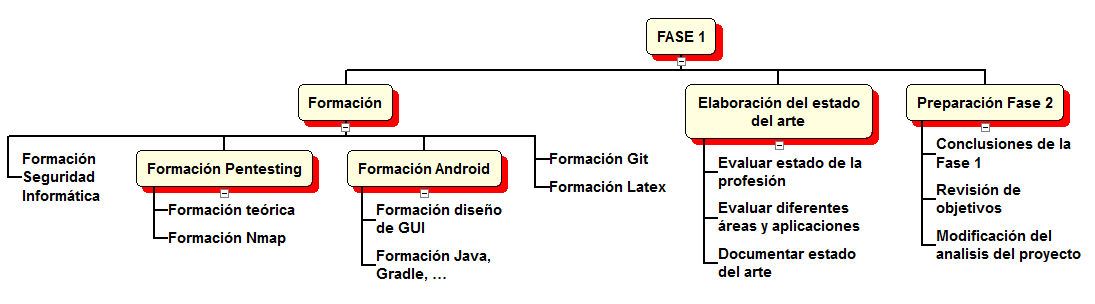
\includegraphics[height=150px]{TFG_EDT_FASE_1}
		\caption{EDT de la Fase 1}
		\label{fig:edt1}
	\end{figure}

\end{landscape}

\subsubsection{Fase 2}
El EDT para la Fase 2 quedaría como se muestra en las figura \ref{fig:edt2}.

\begin{figure}[H]
	\centering
	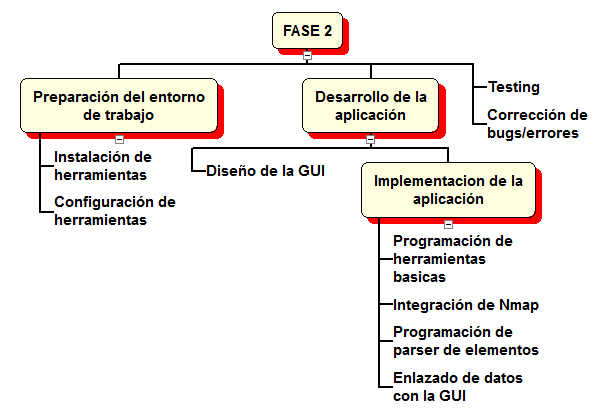
\includegraphics[width=1\textwidth]{TFG_EDT_FASE_2}
	\caption{EDT de la Fase 2}
	\label{fig:edt2}
\end{figure}

\subsection{Agenda del proyecto}
El proyecto se llevara a cabo durante varios meses, comenzando en abril. Se trabajará a media jornada (4 horas) de lunes a viernes, con las siguientes excepciones. Primero, se tendrá en cuneta el calendario de festivos oficiales para aplicar algunas jornadas festivas en cuyos días no se trabajará. Esos días quedan reflejados en la tabla \ref{table:festivos-oficiales}. A esos festivos se les aplica unas excepciones, en las cuales, aun siendo festivo, se trabajará igualmente. Esos festivos en los que se trabaja están indicados en rojo.

\begin{table}[H]
	\centering
	\begin{tabular}{ |c|c| } 
		\hline
		Fecha & Evento \\
		\hline
		1 de Enero & Año nuevo \\
		6 de Enero & Día de Reyes \\
		19 de Marzo & San José \\
		{\color{red} 2 de Abril} & {\color{red} Jueves Santo }\\
		{\color{red} 3 de Abril} & {\color{red} Viernes Santo }\\
		{\color{red} 6 de Abril} & {\color{red} Lunes de Pascua }\\
		28 de Abril & San Prudencio \\
		1 de Mayo & Día del trabajo \\
		{\color{red}25 de Julio} & {\color{red}Santiago Apóstol } \\
		5 de Agosto & Virgen Blanca \\
		15 de Agosto & Asunción de la Virgen \\
		12 de Octubre & Fiesta Nacional de España \\
		8 de Diciembre & Inmaculada Concepción \\
		25 de Diciembre & Navidad \\
		\hline
	\end{tabular}
	\caption{Calendario de días festivos oficial (de Álava)}
	\label{table:festivos-oficiales}
\end{table}

Por otra parte, existen una serie de días en los que se aplica una reducción de la jornada laboral de 4 a 2 horas (en los días considerados laborales), debido básicamente a exámenes. Estos periodos vienen indicados en la tabla \ref{table:reduccion-jornada}.

\begin{table}[H]
	\centering
	\begin{tabular}{ |c|c|c| } 
		\hline
		Nombre del periodo & Fecha de inicio & Fecha de fin \\
		\hline
		Exámenes Convocatoria Ordinaria & 16 de mayo & 23 de mayo \\
		Exámenes Convocatoria Extraordinaria & 27 de junio & 4 de julio \\
		\hline
	\end{tabular}
	\caption{Reducciones de la jornada laboral}
	\label{table:reduccion-jornada}
\end{table}

En base a dicho calendario, la fecha estimada de finalización del proyecto es del 24 de Julio.

\subsection{Tareas}
El EDT completo de tareas, al que se añaden la fase inicial de objetivos del proyecto, y toda la fase final de elaboración de la memoria, presentación y la defensa quedaría de la siguiente manera.
\begin{numbered}
	\setcounter{numberedi}{-1} %Para empeza a contar desde 0
	
	\item Análisis del proyecto
	\begin{numbered}
		\item Objetivos del proyecto
		\item RF del proyecto
	\end{numbered}
	
	\item FASE 1
	\begin{numbered}
		
		\item Formación
		\begin{numbered}
			\item Formación seguridad informatica
			\item Formación Pentesting
			\begin{numbered}
				\item Formación Teórica
				\item Formación NMap
			\end{numbered}
			\item Formación Android
			\begin{numbered}
				\item Formación Diseño de GUI
				\item Fornacion Java, Gradle, ...
			\end{numbered}
			\item Formación Git
			\item Formacion Latex
		\end{numbered}
		
		\item Elaboración del estado del arte
		\begin{numbered}
			\item Evaluar estado de la profesión
			\item Evaluar diferentes areas y aplicaciones
			\item Documentar estado del arte
		\end{numbered}
		
		\item Preparación de la Fase 2
		\begin{numbered}
			\item Conclusiones de la Fase 1
			\item Revisión de objetivos
			\item Modificación del análisis del proyecto
		\end{numbered}
	\end{numbered}
	
	\item FASE 2
	\begin{numbered}
		\item Preparación del entorno de trabajo
		\begin{numbered}
			\item Instalación de herramientas
			\item Configuracion de herramientas
		\end{numbered}
		
		\item Desarrollo de la aplicación
		\begin{numbered}
			\item Diseño de la GUI
			\item Implementacion de la apicación
			\begin{numbered}
				\item Programación de herramientas básicas
				\item Integración de Nmap
				\item Programación de parser de elementos
				\item Enlazado de datos con la GUI
			\end{numbered}
			\item Testeo
			\item Corrección de bugs/errores
		\end{numbered}
	\end{numbered}
	
	\item Elaboración de la memoria
	\begin{numbered}
		\item Integración del estado del arte
		\item Documentación de la aplicación desarrollada
		\item Resumen de la memoria
		\item Elaborar presentación
		\item Preparación de la defensa
	\end{numbered}
	
	\item Reuniones periódicas
\end{numbered}

A continuación se explica mediante una breve definición en que consiste cada tarea, ademas de especificar su duración en horas.

\taskframe
	{0.1}
	{Objetivos del proyecto}
	{Definir los objetivos que tiene que cumplir el TFG}
	{5}
\taskframe
	{0.2}
	{RF del proyecto}
	{Definir, en base a los objetivos del proyecto, los Requisitos funcionales concretos del proyecto}
	{5}
\taskframe
	{1.1.1}
	{Formación seguridad informática}
	{Familiarizarse con el amplio entorno de la seguridad informática y comprender las diferentes áreas, objetivos y el estado de dicho campo}
	{30}
\taskframe
	{1.1.2.1}
	{Formación Teórica}
	{Familiarizarse con los conceptos de Pentesting, las diferentes técnicas usadas y las diferentes fases del proceso de Pentesting}
	{20}
\taskframe
	{1.1.2.2}
	{Formación NMap}
	{Familiarizarse con el entorno de NMap, como implementarlo, usarlo para obtener información y de que formas se puede obtener información estructurada y organizada para su posterior uso}
	{10}
\taskframe
	{1.1.3.1}
	{Formación Diseño de GUI}
	{Aprender a usar herramientas de diseño de GUI, diferentes patrones de Diseño en sistemas Android, y el uso de IDEs o herramientas para desarrollar dichas GUIs}
	{10}
\taskframe
	{1.1.3.2}
	{Formación Java, Gradle, ...}
	{Aprender sobre el uso de Java para desarrollar aplicaciones Android, diferentes clases, utilidades o conceptos recurrentes en la programación para Android}
	{15}
\taskframe
	{1.1.4}
	{Formación Git}
	{Aprender el uso de dicho sistema de control de versiones para llevar un control riguroso del desarrollo del proyecto y de la aplicación}
	{5}
\taskframe
	{1.1.5}
	{Formación Latex}
	{Aprender diferentes conceptos de \LaTeX para elaborar tanto el estado del arte como el propio informe de la manera mas clara y elegante posible}
	{5}
\taskframe
	{1.2.1}
	{Evaluar estado de la profesión}
	{Analizar los diferentes campos de la profesión, las necesidades mas demandadas y los diferentes perfiles de profesionales dentro del campo}
	{5}
\taskframe
	{1.2.2}
	{Evaluar diferentes áreas y aplicaciones}
	{Evaluar las necesidades concretas a nivel técnico, las aplicaciones mas usadas y las virtudes y carencias de éstas}
	{10}
\taskframe
	{1.2.3}
	{Documentar estado del arte}
	{Elaborar la documentación en base a toda la información recogida para obtener un elaborado estado del arte}
	{5}
\taskframe
	{1.3.1}
	{Conclusiones de la Fase 1}
	{Elaborar una serie de conclusiones en función a todo el estudio realizado sobre el campo de la seguridad informática}
	{5}
\taskframe
	{1.3.2}
	{Revisión de objetivos}
	{Revisión de los objetivos y los requisitos funcionales de la aplicación a desarrollar en función a todo lo investigado}
	{5}
\taskframe
	{1.3.3}
	{Modificación del análisis del proyecto}
	{Modificar la parte de análisis del proyecto realizada anteriormente, antes de comenzar con la Fase 1}
	{5}					
\taskframe
	{2.1.1}
	{Instalación de herramientas}
	{Instalación de todo lo necesario para desarrollar la aplicación}
	{5}
\taskframe
	{2.1.2}
	{Configuración de herramientas}
	{Configuración de todas las herramientas para que el desarrollo de la aplicación sea lo mas cómodo posible}
	{5}
\taskframe
	{2.2.1}
	{Diseño de la GUI}
	{Diseñar una interfaz gráfica clara y sencilla de usar para interactuar con las funciones a implementar}
	{15}
\taskframe
	{2.2.2.1}
	{Programación de herramientas básicas}
	{Programar herramientas básicas para el escaneo de redes}
	{10}
\taskframe
	{2.2.2.2}
	{Integración de Nmap}
	{Integrar el núcleo de NMap en la aplicación para poder hacer uso de toda su funcionalidad}
	{10}
\taskframe
	{2.2.2.3}
	{Programación de parser de elementos}
	{Elaborar un puente entre NMap y la aplicación para obtener los datos de NMap y poder usarlos en la aplicación de la manera más organizada posible}
	{20}
\taskframe
	{2.2.2.4}
	{Enlazado de datos con la GUI}
	{Enlazar los datos con las diferentes vistas a través de diversos controladores, para poder visualizar e interactuar con ellos}
	{15}
\taskframe
	{2.2.3}
	{Testing}
	{Una vez desarrollada la aplicación, realizar un amplio testeo para comprobar que funciona correctamente}
	{10}
\taskframe
	{2.2.4}
	{Corrección de bugs/errores}
	{En base a los errores detectados en el testeo, implementar las correcciones a dichos fallos}
	{15}
\taskframe
	{3.1}
	{Integración del estado del arte}
	{Integrar el estado del arte desarrollado dentro de la memoria}
	{5}
\taskframe
	{3.2}
	{Documentación de la aplicación desarrollada}
	{Elaborar en base a todo el proceso de desarrollo una documentación clara sobre la aplicación e integrarla en la memoria}
	{15}
\taskframe
	{3.3}
	{Resumen de la memoria}
	{Terminar la elaboración de la memoria, añadiendo las diferentes secciones necesarias y el formato correspondiente}
	{5}
\taskframe
	{3.4}
	{Elaborar presentación}
	{Elaborar la presentación en diapositivas que se usará en la defensa ante el tribunal}
	{5}
\taskframe
	{3.5}
	{Preparación de la defensa}
	{Preparar la defensa ante el tribunal en función a la documentación elaborada}
	{10}
\taskframe
	{4}
	{Reuniones periódicas}
	{Reuniones periódicas con el director del TFG para llevar un control del desarrollo del proyecto}
	{15}

\subsection{Entregables}

\subsubsection{Fase 1}
El entregable de la Fase 1 consistirá en un estado del arte redactado sobre el campo de la seguridad informática, enfocándose en el área del pentesting.

\subsubsection{Fase 2}
El entregable de la Fase 1 consistirá en una aplicación elaborara, que sirva como herramienta para el escaneo de redes informáticas. La aplicación, elaborada para Android, esta correctamente empaquetada, con los posible fallos corregidos y además dispondrá de una GUI sencilla de usar.



\subsection{Cronograma}
El cronograma completo, con las dos fases, como se muestra en las figuras \ref{fig:gantt0}, \ref{fig:gantt1}, \ref{fig:gantt2} y \ref{fig:gantt3} respectivamente.

\begin{figure}[H]
	\centering
	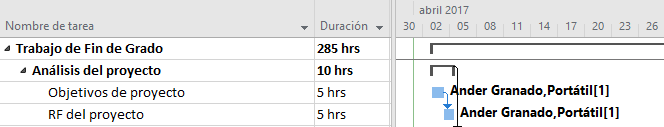
\includegraphics[width=1\textwidth]{TFG_GANTT_FASE_0}
	\caption{Cronograma de la fase inicial}
	\label{fig:gantt0}
\end{figure}

\begin{landscape}

\begin{figure}[H]
	\centering
	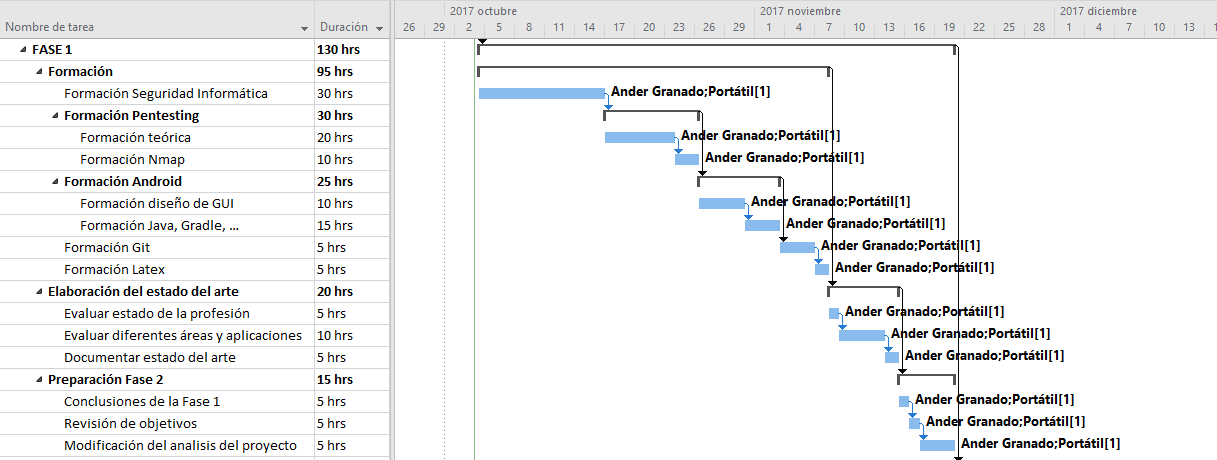
\includegraphics[height=250px]{TFG_GANTT_FASE_1}
	\caption{Cronograma de la Fase 1}
	\label{fig:gantt1}
\end{figure}

\begin{figure}[H]
	\centering
	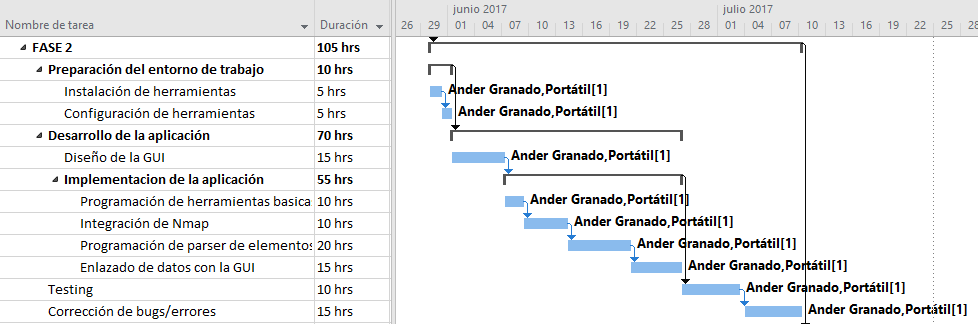
\includegraphics[height=200px]{TFG_GANTT_FASE_2}
	\caption{Cronograma de la Fase 2}
	\label{fig:gantt2}
\end{figure}

\end{landscape}

\begin{figure}[H]
	\centering
	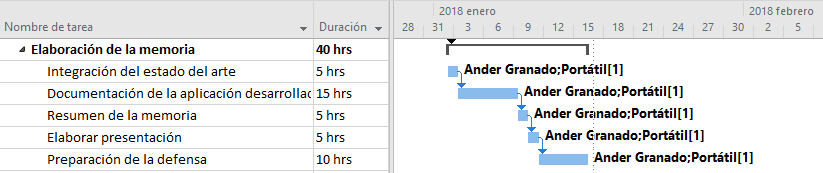
\includegraphics[width=1\textwidth]{TFG_GANTT_FASE_3}
	\caption{Cronograma de la elaboración de la memoria}
	\label{fig:gantt3}
\end{figure}





%------------------------------------------------------------------------------

\section{Gestión de costos}
{\color{red} Poner los recursos que se necesitan.}

\begin{table}[H]
	\centering
	\begin{tabular}{ |l|r| } 
		\hline
		Concepto & Coste \\
		\hline
		Ander Granado & 14,00 \euro/h \\
		\hline
	\end{tabular}
	\caption{Recursos de trabajo}
	\label{table:recursos-trabajo}
\end{table}

\begin{table}[H]
	\centering
	\begin{tabular}{ |l|r| } 
		\hline
		Concepto & Coste \\
		\hline
		Ordenador portátil & 700,00 \euro \\
		BQ Aquaris M5 & 250,00 \euro \\
		\hline
	\end{tabular}
	\caption{Recursos materiales (hardware)}
	\label{table:recursos-materiales}
\end{table}

\begin{table}[H]
	\centering
	\begin{tabular}{ |l|r|r| } 
		\hline
		Concepto & Coste & Numero de licencias \\
		\hline
		Windows 10 & 135,00 \euro \cite{precio-win10} & 1 \\
		Project 2016 & 1369,00 \euro \cite{precio-project} & 1 \\
		WBS Chart Pro & 187,50 \euro \cite{precio-wbs} & 1 \\
		Ubuntu 16.04 & 0,00 \euro & 1 \\
		TeX Studio & 0,00 \euro & 1 \\
		Android Studio & 0,00 \euro & 1 \\
		NMap & 0,00 \euro & 1 \\
		Git & 0,00 \euro & 1 \\
		GitHub & 0,00 \euro & 1 \\
		\hline
	\end{tabular}
	\caption{Recursos materiales (software)}
	\label{table:recursos-software}
\end{table}

\begin{table}[H]
	\centering
	\begin{tabular}{ |l|r|r|r|r|r| } 
		\hline
		Concepto & Trabajo (h) & Trabajo horas extra & Coste & Coste horas extra & Importe \\
		\hline
		Ander Granado & 285 & 0 & 14,00 \euro/h & 0 & 4.044,00 \euro \\
		\hline
	\end{tabular}
	\caption{Costo de recursos de trabajo}
	\label{table:costo-recursos-trabajo}
\end{table}

\begin{table}[H]
	\centering
	\begin{tabular}{ |l|r|r|r| } 
		\hline
		Concepto & Unidades & Coste & Importe \\
		\hline
		Ordenador portátil & 1 & 1,50 \euro/uso & 29 x 1,50 \euro \space= 43,50 \euro \\
		BQ Aquaris M5 & 1 & 1,50 \euro/uso & 7 x 1,50 \euro \space= 10,50 \euro \\
		\hline
		TOTAL & & & 54,00 \euro\\ 
		\hline
	\end{tabular}
	\caption{Costo de recursos materiales}
	\label{table:costo-recursos-trabajo}
\end{table}

\begin{table}[H]
	\centering
	\begin{tabular}{ |l|r|r|r|r|r| } 
		\hline
		Concepto & Coste unitario & T. de amortización & C. U. amortización & T. de uso & Importe \\
		\hline
		Ordenador portátil & 700,00 \euro & 4800 horas & & & \\
		BQ Aquaris M5 & 250,00 \euro & 4800 horas & & & \\
		Windows 10 & 135,00 \euro & 4800 horas & & & \\
		Microsoft Project 2016 & 1369,00 \euro & 4800 horas & & & \\
		WBS Chart Pro & 187,50 \euro & 4800 horas & & & \\
		Ubuntu 16.04 & 0,00 \euro & 4800 horas & & & \\
		TeX Studio & 0,00 \euro & 4800 horas & & & \\
		Android Studio & 0,00 \euro & 4800 horas & & & \\
		NMap & 0,00 \euro & 4800 horas & & & \\
		Git & 0,00 \euro & 4800 horas & & & \\
		GitHub & 0,00 \euro & 4800 horas & & & \\
		\hline
	\end{tabular}
	\caption{Amortizaciones de hardware y de software}
	\label{table:amortizaciones}
\end{table}

\begin{table}[H]
	\centering
	\begin{tabular}{ |c|c| } 
		\hline
		Concepto & Importe \\
		\hline
		Recursos de Trabajo (R.T.) & 4.044,00 \euro \\
		Recursos Materiales (R.M.) & 4.044,00 \euro \\
		\hline
	\end{tabular}
	\caption{Total presupuesto}
	\label{table:total-presupuesto}
\end{table}

\subsection{Presupuesto}
{\color{red} Todas las tablas y así, todo lo dado en la asignatura de Mari Carmen.}

%------------------------------------------------------------------------------

\section{Gestión de riesgos}

\subsection{Fase 1}
{\color{red} Poner los diferentes riesgos de la Fase 1. En esta fase son pocos o ninguno, por el carácter teórico de la fase.}

\subsubsection{Explicación y plan de contingencia}
{\color{red} Explicar dichos riesgos. Poner por puntos. Puntos como descripción, peligrosidad, y medidas preventivas o para corregir. Nada de párrafos.}

\subsection{Fase 2}
{\color{red} Poner los diferentes riesgos de la Fase 2. En esta fase los riesgos son mucho mayores, ya que puede haber desde complicaciones a la hora de programar, limitaciones por no ser root,... Mil historias.}

\subsubsection{Explicación y plan de contingencia}
{\color{red} Explicar dichos riesgos. Poner por puntos. Puntos como descripción, peligrosidad, y medidas preventivas o para corregir. Nada de parrafos.}

